\section{希格斯对衰变}
希格斯粒子的寿命只有$1.56\times10^{-22}~$s,在对撞顶点即衰变,表\ref{fig:HH_br}总结了$hh$的主要衰变道的分支比。在\RunOne ,ATLAS研究过$b\bar{b}b\bar{b}$\cite{Aad:2015uka},
$b\bar{b}\gamma\gamma$~\cite{Aad:2014yja},$b\bar{b}\tau^{+}\tau^{-}$和$WW^{*}\gamma\gamma$,均没有观测到数据与预期的明显偏差。
对于非共振态模式,其截面上限为0.69 pb,对应$\kappa<$70。
共振态模式的联合拟合截面上限总结在图\ref{fig:HH_run1_combined}。
\begin{figure}[h]
\centering
 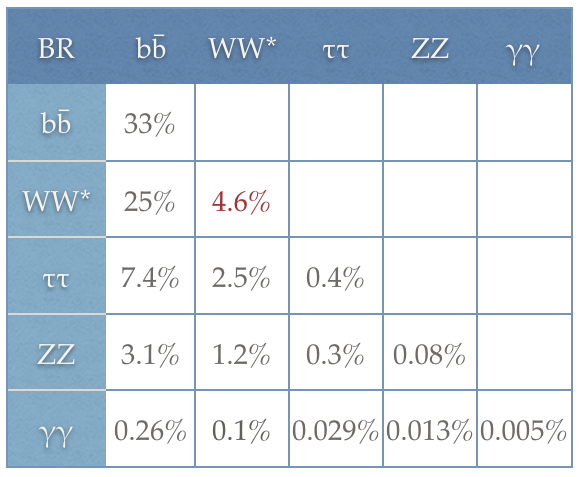
\includegraphics[width=0.75\textwidth]{fig/HH_br.png}
  \caption{$hh$主要衰变道分支比,计算时假设$m_h$=125 GeV。}
  \label{fig:HH_br}
\end{figure}

\begin{figure}[h]
\centering
 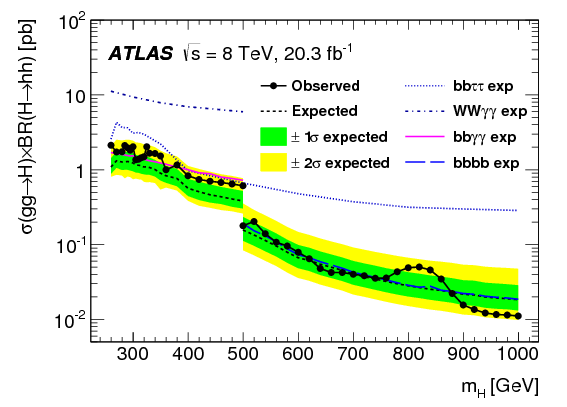
\includegraphics[width=0.85\textwidth]{fig/HH_run1_combined.png}
\caption{在8 TeV质心系能量时$\sigma(gg\rightarrow H)\times\text{BR}(H\rightarrow hh)$的95\%置信度下的观测上限值与期
望上限值,结果联合拟合了$b\bar{b}\tau\tau$, $WW^*\gamma\gamma$, $b\bar{b}\gamma\gamma$以及$b\bar{b}b\bar{b}$分析道。绿色和黄色区分别表示期望上限值的$\pm 1\sigma$和$\pm 2\sigma$,500 GeV以上的提升得益于$b\bar{b}b\bar{b}$的加入。}
\label{fig:HH_run1_combined}
\end{figure}

\RunTwo ATLAS和CMS均继续希格斯对的寻找,以下对一些衰变道及其最新结果作出简要概述:
\begin{itemize}
 \item $b\bar{b}b\bar{b}$:它具有最大的衰变分支比,是$hh$搜寻的主要分析道,能够重建Higgs以及$X$的质量,但是其分辨率
受限于$b$喷注重建及鉴别。在低$m_X$区,因为$b$喷注触发效率太低,其显著性较低;但是在高$m_X$区,两个$b$喷注倾向合并,可以重建两个large-$R$~$b$喷注,而且得
益于提高的$b$喷注触发效率,其显著性得到提高。目前ATLAS给出的SM $hh$最新截面上限为13倍SM预期\cite{Aaboud:2018knk}(95\%置信度,以下相同),CMS对共振态模式进行了寻找\cite{Sirunyan:2018zkk}。
 \item $b\bar{b}W^{+}W^{-}$:具有第二大分支比,但是$t\bar{t}$本底限制了显著性。SM $hh$寻找的ATLAS最新结果为300倍SM预期\cite{Aaboud:2018zhh},而CMS最新结果为79倍SM预期\cite{Sirunyan:2017guj}。
 \item $b\bar{b}\gamma\gamma$:虽然截面不大,但是受益于较干净的双光子本底以及很好的光子分辨,在低$m_X$区有显著优势,
 但在高质量区,双光子的合并对光子鉴别造成影响,使得显著性下降。SM $hh$寻找的ATLAS最新结果为22倍SM预期\cite{Aaboud:2018ftw},CMS则为24倍预期\cite{Sirunyan:2018iwt}。
 \item $b\bar{b}\tau^{+}\tau^{-}$:该道与$b\bar{b}b\bar{b}$和$b\bar{b}\gamma\gamma$具有相当的显著性,尤其是在低$m_X$区,其主要挑战是赝$\tau$的
本底处理。SM $hh$寻找的ATLAS最新结果为12.7倍SM预期\cite{Aaboud:2018sfw},CMS则为30倍预期\cite{Sirunyan:2017djm}。
 \item $WW^{*}\gamma\gamma$:该道与上述衰变道相比具有较差的显著性,但是得益于双光子以及轻子化衰变的$W$玻色子,
本底较少,是$hh$搜寻的重要补充。ATLAS实验给出的SM $hh$最新结果为162倍SM预期\cite{Aaboud:2018ewm}。
 \item $WW^{*}WW^{*}$:本章$hh$分析的研究题目,关于此道已有唯象研究\cite{4WTheory},但在ATLAS是首次寻找。
它具有较大衰变分支比,以轻子末态为信号特征可极大压低QCD本底。
 \item $WW^{*}\tau\tau, \tau\tau\gamma\gamma, \tau\tau\tau\tau, b\bar{b}ZZ, WWZZ$:这些衰变道的分支比都很小,均不能
或者部分重建Higgs,还未公开发表过结果。
 但是随着ATLAS累积更多的数据,使用单举策略\footnote{$WW^{*}\gamma\gamma$和$WW^{*}WW^{*}$也纳入其中},即以它们的衰变
物进行分类,如轻子数,
 不明显关注$hh$衰变中间态,而后进行优化,最后联合拟合得出结果,也许可以为$hh$搜寻作出重要贡献。
\end{itemize}

本章论述通过$WW^{*}WW^{*}$衰变道寻找$hh$(以及$SS$)产生模式,在此分析道,目前已开展三个末态分析,
包括相同电荷双轻子(2LSS),三轻子(3L)和四轻子(4L),本章将给出2LSS衰变道分析的研究过程及结果,并联合三个末态给出
统计结果。
